\documentclass{article}[11pt]

\usepackage{amsmath}
\usepackage{amsfonts}

\usepackage{graphicx}
\graphicspath{{../fig/}} 								% Path to a folder where all pictures are located

\usepackage{fullpage}

\title{Machine Learning -- Assignment 9}
\author{Weipeng He and Sathyanarayanan}

\begin{document}

\maketitle

\section{}
\subsection{}
With the labeled data, we evaluate precision of the clustering as same as for classification, while we need to find the best assignment of the clustering first. Formally, let $\mathcal{X} = {X_1, X_2, \dots, X_k}$ be the clusters, $\mathcal{Y} = {Y_1, Y_2, \dots, Y_k}$ be the standard classes, $\mathcal{F} = \left\{f:\mathcal{X}\rightarrow\mathcal{Y} | f \text{ is bijection}\right\}$ be the all possible assignment from clusters to classes. We define the score of a clustering as:
\[ \frac{\max_{f \in \mathcal{F}} \sum_{i=1}^{k} \left| X_i \cap f(X_i) \right|}{\sum_{i=1}^{k} \left| Y_i \right|}  \]

\subsection{}
While, if the data are not labeled. We use \emph{Dunn Index} as the criterion:
\[ DunnIndex = min_{i \neq j} \frac{\delta(X_i,X_j)}{max_{l} \Delta_l} \]
where $\delta(\cdot,\cdot)$ is the inter-cluster distance (here we use average distance between points in different clusters), and $\Delta_l$ is the intra-cluster distance of cluster $l$ (here we use the average distance between all points in the cluster).

\subsection{}
The results of different distance measures are shown as follow: 
\begin{center}
\begin{tabular}[h]{c|ccc}
  \hline
  Distance & Euclidean & City Block & Cosine \\ \hline
  Precision &  0.845000 & 0.840000 & 0.920000 \\
  Dunn Index & 0.941602 & 1.130539 & 1.112118 \\ \hline
\end{tabular}
\end{center}

\section{}
\subsection{}
With unnormalized spectural clustering, the embedding is shown as follow:
\begin{center}
  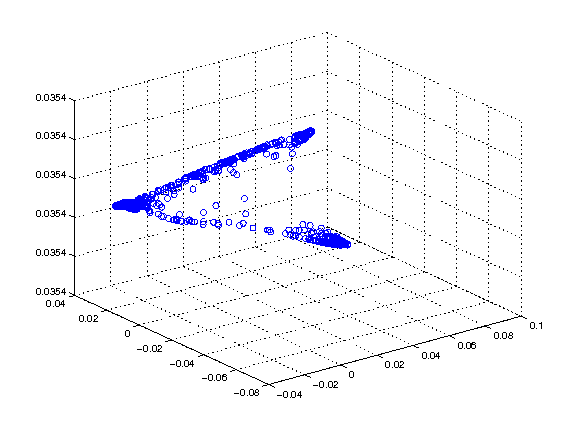
\includegraphics[width=.7\textwidth]{spec}
\end{center}
and normalized spectural clustering:
\begin{center}
  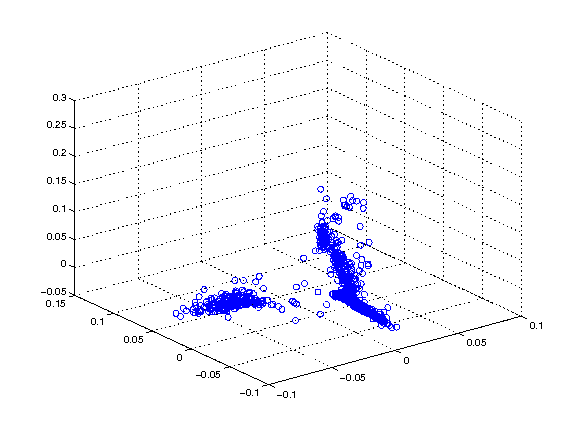
\includegraphics[width=.7\textwidth]{normspec}
\end{center}

The results of spectural clustering: 
\begin{center}
\begin{tabular}[h]{c|ccc}
  \hline
  Method & Spectural & Normalized Spectural \\ \hline
  Precision & 0.990000 & 0.990000 \\
  Dunn Index & 1.200640 & 1.222372 \\ \hline
\end{tabular}
\end{center}

\end{document}
